\renewcommand*{\arraystretch}{1.1}

\subsection*{BI / read / 22}
\label{section:bi-read-22}

\noindent\begin{tabularx}{\queryCardWidth}{|>{\queryPropertyCell}p{\queryPropertyCellWidth}|X|}
	\hline
	query & BI / read / 22 \\ \hline
%
	title & International dialog
 \\ \hline
%
	pattern & \hfill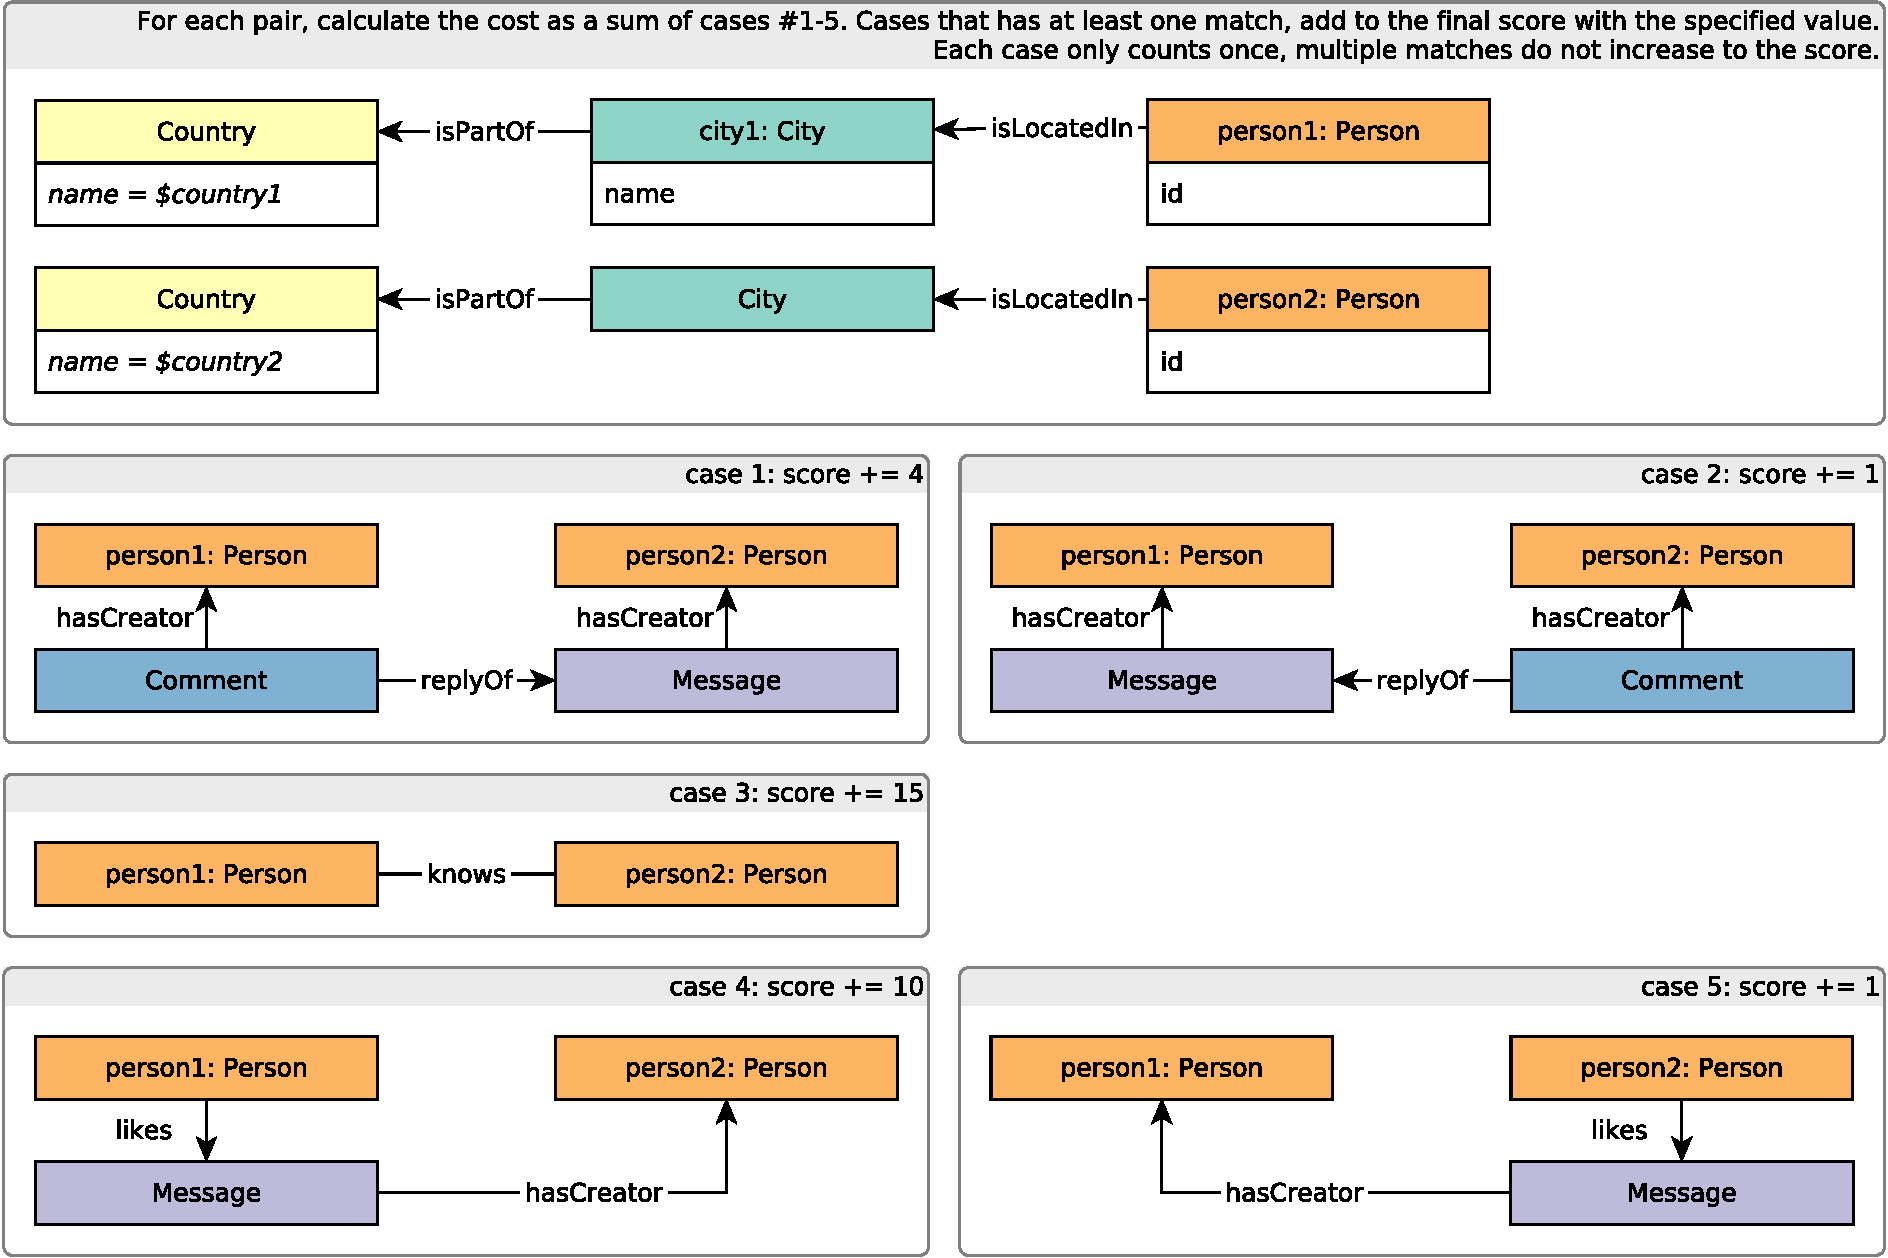
\includegraphics[scale=\patternscale,margin=0cm .2cm]{patterns/bi-read-22}\hfill\vadjust{} \\ \hline
%
	desc. & Consider all pairs of people \texttt{(person1,\ person2)} such that one
is located in a \emph{City} of \emph{Country} \texttt{country1} and the
other is located in a \emph{City} of \emph{Country} \texttt{country2}.

For each \emph{City} of \emph{Country} \texttt{country1}, return the
highest scoring pair.

The score of a pair is defined as the sum of the subscores awarded for
the following kinds of interaction. The initial value is
\texttt{score\ =\ 0}.

\begin{enumerate}
\def\labelenumi{\arabic{enumi}.}
\tightlist
\item
  \texttt{person1} has created a reply \emph{Comment} to at least one
  \emph{Comment} or \emph{Post} by \texttt{person2}:
  \texttt{score\ +=\ 4}
\item
  \texttt{person1} has created at least one \emph{Post} or
  \emph{Comment} that \texttt{person2} has created a reply
  \emph{Comment} to: \texttt{score\ +=\ 1}
\item
  \texttt{person1} and \texttt{person2} \emph{know} each other:
  \texttt{score\ +=\ 15}
\item
  \texttt{person1} liked at least one \emph{Post} or \emph{Comment} by
  \texttt{person2}: \texttt{score\ +=\ 10}
\item
  \texttt{person1} has created at least one \emph{Post} or
  \emph{Comment} that was liked by \texttt{person2}:
  \texttt{score\ +=\ 1}
\end{enumerate}

Consequently, the maximum score a pair can obtain is:
\texttt{4\ +\ 1\ +\ 15\ +\ 10\ +\ 1\ =\ 31}
 \\ \hline
%
	
		params &
		\innerCardVSpace{\begin{tabularx}{\attributeCardWidth}{|>{\paramNumberCell}c|>{\varNameCell}M|>{\typeCell}m{\typeWidth}|Y|} \hline
		$\mathsf{1}$ & country1
 & String
 &  \\ \hline
		$\mathsf{2}$ & country2
 & String
 &  \\ \hline
		\end{tabularx}}\innerCardVSpace \\ \hline
	
%
	
		result &
		\innerCardVSpace{\begin{tabularx}{\attributeCardWidth}{|>{\resultNumberCell}c|>{\varNameCell}M|>{\typeCell}m{\typeWidth}|>{\resultOriginCell}c|Y|} \hline
		$\mathsf{1}$ & person1.id & 64-bit Integer & R &
				 \\ \hline
		$\mathsf{2}$ & person2.id & 64-bit Integer & R &
				 \\ \hline
		$\mathsf{3}$ & city1.name & String & R &
				 \\ \hline
		$\mathsf{4}$ & score & 32-bit Integer & C &
				 \\ \hline
		\end{tabularx}}\innerCardVSpace \\ \hline
	
%
	
		sort		&
		\innerCardVSpace{\begin{tabularx}{\attributeCardWidth}{|>{\sortNumberCell}c|>{\varNameCell}M|>{\directionCell}c|Y|} \hline
		$\mathsf{1}$ & score
 & $\desc
$ &  \\ \hline
		$\mathsf{2}$ & person1.id
 & $\asc
$ &  \\ \hline
		$\mathsf{3}$ & person2.id
 & $\asc
$ &  \\ \hline
		\end{tabularx}}\innerCardVSpace \\ \hline
	%
	%
	CPs &
	\multicolumn{1}{>{\raggedright}l|}{
		\chokePoint{1.4}, 
		\chokePoint{1.6}, 
		\chokePoint{2.1}, 
		\chokePoint{3.1}, 
		\chokePoint{3.3}, 
		\chokePoint{5.1}, 
		\chokePoint{5.2}, 
		\chokePoint{5.3}
		} \\ \hline
	%
	%
\end{tabularx}
\queryCardVSpace